\section{Task 1: Normalisation}

Figure 1 below shows part of a spreadsheet used by a tavern which allows customers to book rooms for events and functions. Each row represents a booking.

\begin{figure}[H]
\centering
\caption{Tavern Bookings}
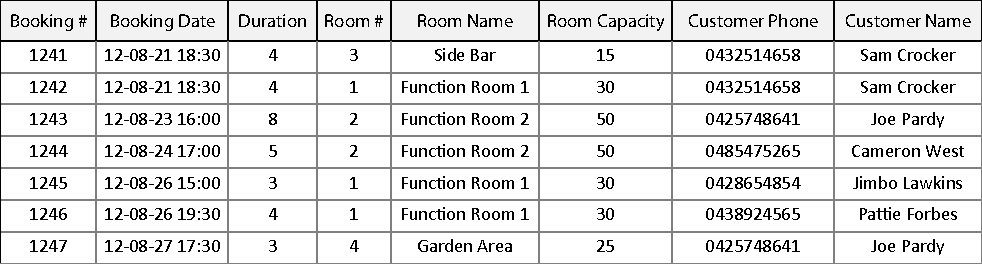
\includegraphics[scale=1]{./img/task1.pdf}
\end{figure}

\subsection*{Assumptions}

\begin{itemize}
\item The pub currently identifies customers by their phone number
\item A room cannot have multiple bookings at the same time
\end{itemize}

\subsection{0NF: Unnormalised}

R1 = (CustomerPhone, CustomerName, {Booking\#, BookingDate, Duration, Room\#, RoomName, RoomCapacity})

\subsection{1NF: First normal form}

\sout{R1 = (\textbf{\underline{CustomerPhone}}, CustomerName, \{\textbf{\underline{Booking\#}}, BookingDate, Duration, Room\#,RoomName, RoomCapacity\})}
\\\\
R11 = (\textbf{\underline{CustomerPhone}}, CustomerName)
\\\\
R12 = (\textbf{\underline{Booking\#}}, BookingDate, Duration, Room\#, RoomName, RoomCapacity, \emph{CustomerPhone})

\subsection{2NF: Second normal form}

No partial dependencies, already 2NF.
\\\\
R11 = (\textbf{\underline{CustomerPhone}}, CustomerName)
\\\\
R12 = (\textbf{\underline{Booking\#}}, BookingDate, Duration, Room\#, RoomName, RoomCapacity, \emph{CustomerPhone})

\subsection{3NF: Third normal form}

R11 = (\textbf{\underline{CustomerPhone}}, CustomerName)
\\\\
\sout{R12 = (\textbf{\underline{Booking\#}}, BookingDate, Duration, Room\#, RoomName, RoomCapacity, \emph{CustomerPhone})}
\\\\
R121 = (\textbf{\underline{Booking\#}}, BookingDate, Duration, \emph{Room\#}, \emph{CustomerPhone})
\\\\
R122 = (\textbf{\underline{Room\#}}, RoomName, RoomCapacity)

\subsection{Named relations}

Customer = (\textbf{\underline{CustomerPhone}}, CustomerName)
\\\\
Booking = (\textbf{\underline{Booking\#}}, BookingDate, Duration, \emph{Room\#}, \emph{CustomerPhone})
\\\\
Room = (\textbf{\underline{Room\#}}, RoomName, RoomCapacity)